\chapter{Manage Globus Groups}
Globus allows you to create and manage groups of Globus users and share files and 
folders with these groups.

\begin{center}
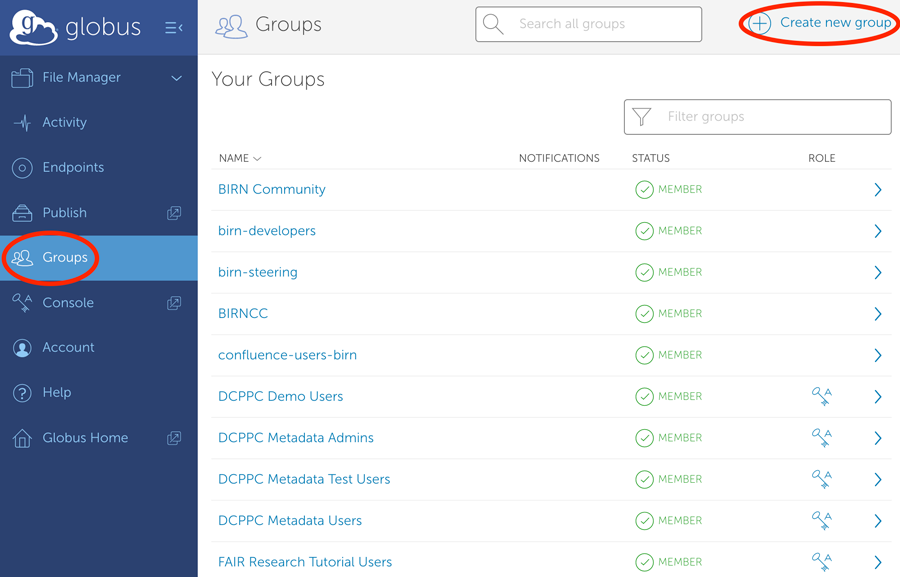
\includegraphics[width=0.5\textwidth]{img/groups-1.png}
\end{center}

\begin{itemize}
\item Click \emph{Groups} in the left-side command pane to open the Your Groups page. 
You will see a list of all the groups you are a member of, including those you 
administer or manage. To search for a group you belong to, type part of its name 
in the Filter groups field above the list.
\item Click \emph{Create new group} to create a group.
\item Type a name for the group. You can also enter a description that tells 
prospective members about the group. Then click \emph{Create Group}.
\item After creating a group, Globus will return you to the \emph{Your Groups} page. 
Click the right arrow next to the newly created group.
\item Click \emph{Invite Others} to invite other users to the group.
You can invite others to the group by entering email addresses or by searching 
for Globus identities. Globus will send each person an email that includes a link 
for accepting the invitation to the group.
\begin{itemize}
\item Invite by email address: Enter the email address for the person you wish to 
invite and click \emph{Add}. This is a good option to use for members who don not 
yet have a Globus account.
\item Invite by Globus identity: Enter all or part of the person's name or email 
address and press \emph{Enter} to search for a current Globus identity. Select 
the user you wish to invite from the search results.
\end{itemize}
\item Click the \emph{Members} tab to view users who have been invited or who 
are already members of the group. The \emph{Status} field shows the membership 
status of each user, and the \emph{Role} field shows each user's role in the group. 
The \emph{Administrator} in the group can change any user's role or status in the 
group, including removing a user, by clicking the right arrow next to the user's name.
\item Click \emph{the Settings} tab to view the group's settings and policies. 
These policies control who can see the group and its membership list, how new 
users are added to the group, and related privileges. Click \emph{Edit Policies} 
to change any of these policies.
\end{itemize}

%%% Local Variables:
%%% mode: latex
%%% TeX-master: "intro-Globus"
%%% End:
